\chapter{Sensitivity of spin-aligned searches for neutron star-black hole systems}

Current search methods are restricted to systems with quasi-circular orbits and only the dominant mode of the gravitational wave signals. These assumptions degrade the sensitivity for precessing NSBH mergers whose detections provides insights into their formation history. In this chapter, we explore our study of the sensitivity of current search methods for fully precessing NSBH mergers with higher-order modes of GW emission. We also explore how much current search assumptions affect the future observatories. Finally, we estimate the loss in sensitivity for an idealized precessing search.  The aim of this work is to identify the regions of parameter space strongly biased by the current searches and to motivate a target precessing search in those regions with current and future observatories.

\section{Introduction}
In the previous chapter, we discussed eccentricity as a signature of a binary's formation channel. Another signature is the spins of the components in a merger.  In scenarios where the binary components evolve together from their main sequence phase (like in the case of binary neutron stars or some black hole binaries), the spins are expected to be relatively well-aligned with the orbital angular momentum. This alignment can be due to the tidal interactions and mass transfer processes in the binary’s evolutionary history, which tend to align the spin axes of the components with the orbit. Conversely, in dense stellar environments like globular clusters or galactic nuclei, binaries can be formed through dynamical interactions. In such scenarios, the spins of the components are more likely to be misaligned with the orbital angular momentum which causes spin-induced precession of the binary orbit. This misalignment occurs because the binary components have independent evolutionary histories and are brought together by chance encounters rather than having evolved together. 

The latest catalogs of compact-object mergers reveal that a small number of these mergers display precession or higher-order modes. Notably, the BBH merger GW200129 has shown compelling signs of precession. Similarly, significant indications of higher-order mode emissions were observed in the events GW190814 and GW190412. Additionally, the ring-down analysis of GW190521 points to the presence of a less dominant mode.

The existing observations of NSBH and BBH mergers poses a challenge to different formation pathways and population synthesis models. Significant uncertainties in these models stem from the incomplete understanding of the binary environments such as distribution of stellar metallicity and physical process such as the dynamics of natal kicks. Identifying precessing NSBH mergers could play a crucial role in refining these models. Search strategies usually operate under the assumption that the spins of compact objects align with their orbital angular momentum, the orbits of these binaries are nearly circular, and only the primary mode $(l, m) = (2, 2)$ of gravitational wave emission is detectable. However, given that NSBH sources often have significant mass differences, it's anticipated that they could exhibit important higher-order modes. Moreover, if their black holes are rapidly spinning, noticeable precession could occur. Ignoring these factors in search methodologies might lead to pronounced biases in observations.  

Measuring spin precession presents significant challenges, particularly due to the detection of most sources at minimal inclination angles []. Furthermore, various studies indicate that deducing the spin precession parameter is complex, often influenced heavily by prior assumptions. Additionally, the substantial systematic differences in waveforms could lead to biased results in estimating the binary parameters. Measuring the higher-order modes of the signal alleviates some of the problems -- sub-dominant modes can carry information on spin-precession and including them in analysis helps break the mass-spin degenaracies [].

Past research has explored the efficacy of searches that focus solely on the dominant-mode of precessing events, as well as the biases that arise from overlooking precession and higher-order modes in binary black hole searches. These specialized searches demand a significantly higher number of templates more than $\sim 10\times$ compared to standard analyses. Due to the increase in the number of templates, such analyses produce a higher rate of false alarms at a fixed signal-to-noise (SNR) threshold. Thus, improvement in searches is driven by two competing effects -- higher SNR from precessing waveforms and larger trials factor. [] have found that searches for binaries with comparable component masses or near face-on systems do not benefit from incorporating misaligned spins or higher modes. However, up to $\sim 25\%$ of NSBH systems might be missed by aligned-spin searches. 

Modeling fast and accurate inspiral-merger-ringdown waveforms for fully precessing signals with relevant sub-dominant modes is an active field. There has been significant improvements to these models since the above mentioned studies were performed. In this work, we use the state-of-art precessing IMR waveforms to compare the sensitivity of spin aligned searches in Advanced LIGO, $A^{\#}$, LIGO Voyager and Cosmic Explorer. We determine the fraction of sources that would be detected by a dominant-mode, aligned-spin search compared to the ideal search that fully accounts for precession and higher-order mode.   


Owing to the inherent challenges associated with each of these methodologies, no search that includes waveforms factoring in precessional effects has been conducted using the data from Advanced LIGO, Advanced Virgo, or KAGRA. Efforts are underway for developing a fully precessing search. A completely different methodology of searching precessing systems using     

\section{Modeling precessing CBC signals with HMs}

Numerous models are available to describe the complete inspiral, merger, and ringdown parts in the gravitational wave signals from compact-binaries. These models are capable of incorporating spin-precession effects and higher-order modes of the signal. They are generally divided into three main categories: phenomenological models, effective one-body numerical relativity (EOBNR) models, and surrogate models. Current searches employ waveform models from both the phenomenological and effective-one body families. Given that our study is focused on the efficacy of model-based searches, we will provide a concise overview of the signal model. 

We revist the quasi-circular CBC signal model that can be characterized by 15 parameters. These parameters are broadly divided as 1. \uline{\textit{Intrinsic parameters}} $\kappa$: the component masses $(m_1, m_2)$ and component spin vectors $(\Vec{\chi_1}, \Vec{\chi_2})$, and the 2. \underline{\textit{Extrinsic parameters}}: the sky-location angles ($\alpha, \delta$) in the frame of the observer, luminosity distance $d_L$, the inclination angle $i$ between the orbital angular momentum \textbf{L} and the line of sight to the observer, polarization angle $\psi$, the time of coalescence $t_c$ and the orbital phase $\phi_c$ of the binary.

The gravitational wave $h(t)$ as seen by a detector is a linear combination of the two gravitational-wave polarization
\begin{align} 
    \begin{aligned}
    h(t) = F_{+}(\alpha, \delta, \psi) & h_{+}(\kappa, i, d_L, \varphi_c; t) \\ & + F_{\times}(\alpha, \delta, \psi)h_{\times}(\kappa, i, d_L, \varphi_c; t),
    \end{aligned}
    \label{Eq:Detector_response}
\end{align}

where the coefficients $F_{+}$ and $F_{\times}$ are the time-independent antenna pattern functions of the detector \cite{Finn:1992xs, Jaranowski:1998qm}. The two polarization are defined in the radiation frame and together they make up the complex strain $H = h_{+} + i h_{\times}$. This complex strain can be further decomposed using the spin-2 weighted spherical harmonics $Y^{-2}_{lm}$ \cite{Spin-weighted-harmonics}
\begin{align}
        \label{Eq:spherical_harmonics}
    H \equiv h_+ + ih_{\times} = \sum_{l\geq2}\sum_{m=-l}^{m=l} Y^{-2}_{l,m}(i, \varphi_c) h_{l,m}(\kappa, d_L ;t-t_c),
\end{align}
where the $h_{l,m}$ are the various \textit{modes} of the GW signal which are function of $\kappa, d_L$ and $t_c$. These various modes  (explicit expression can be found in \cite{Mills:2020thr})) have different contributions to the observed signal via the respective $Y^{-2}_{l,m}(i, \varphi_c)$. The dominant mode $(l,m)$ = (2,2) is the strongest at face-on ($i=0$) or face-off ($i = \pi/2$) configurations and grows fainter with increasing $i$ reaching minimum at $i = \pi/2$. However, significantly inclined binaries can have stronger higher modes. In general for a given mode ($l, m$), we can write  
\begin{align}
    h_{l,m}(\kappa, d_L; t) = A_{l,m}(\kappa, d_L; t)e^{-i\Phi_{l,m}(\kappa;t)},
    \label{Eq:single_mode}
\end{align} 
where $A_{l,m}, \Phi_{l,m}$ are respectively the real amplitude and phase for a given mode. The phase $\Phi_{l, m}$ for each mode is related to the orbital phase as $\Phi_{l,m}(t) = m\phi_{orb}(t)$ up to a good approximation ~\cite{Apostolatos:1994mx}, which depends strongly on the component spins.

The individual modes $h_{l,m}$ are functions of the spin parameters.
We denote the spin angular momenta $\textbf{S}_1 = \vec{\chi}_1 m_1^2$ and $\textbf{S}_2= \vec{\chi}_2 m_2^2$.  In the case of aligned-spin systems, the direction of the orbital angular momentum remains fixed and thus, $\textbf{S}_1 \textbf{S}_2$, and $\textbf{L}$ are parallel. In the case of systems with generically oriented spin vectors, the spins of the compact objects couple with the orbital angular momentum which may cause spin-precession. For such systems, the orbital angular momentum $\textbf{L}$ precesses around the nearly fixed total angular momentum $\textbf{J} = \textbf{S}_1 + \textbf{S}_2 + \textbf{L}$; the inclination angle varies over time. The various spin and orientation angles are shown in the Fig. \ref{fig:precessing_angles}. Note, even though $\textbf{J}$ is considered to be fixed to a good approximation \cite{Apostolatos:1994mx}, there can be rare instances where $\textbf{J}$ can change significantly \cite{Apostolatos:1994mx}. 

\begin{figure}[]
    \centering
    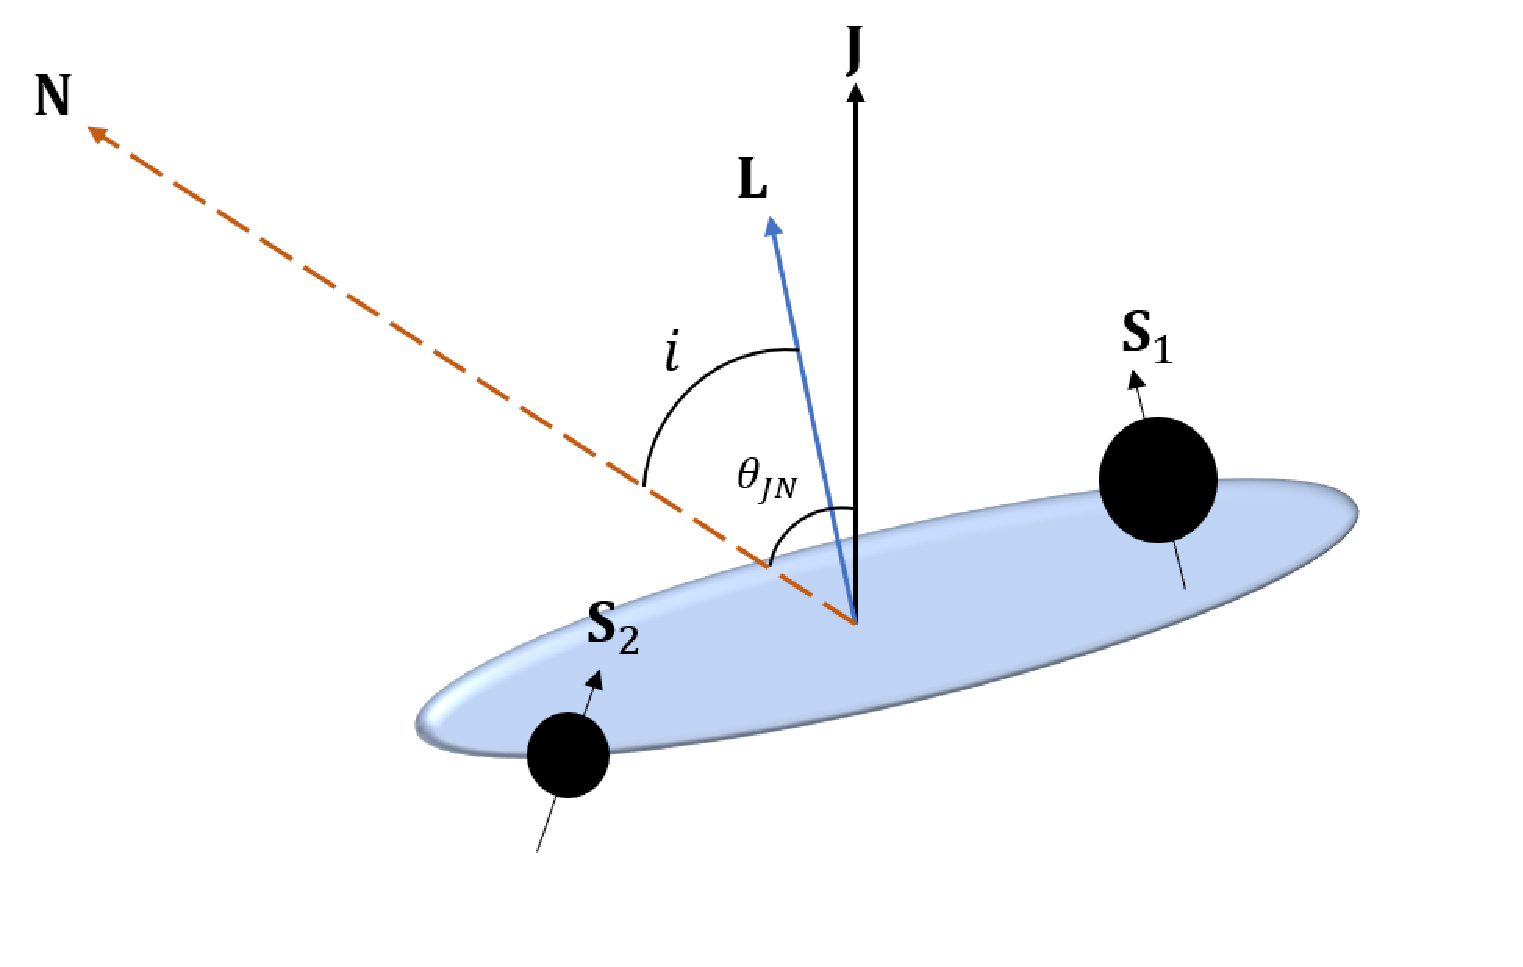
\includegraphics[width=10cm]{figures/HM_and_precession/Precessing_angles.pdf}
    \caption{The angular momentum vectors for a precessing binary. The inclination angle $i$ is defined as the angle between the orbital angular momentum $\textbf{L}$ and the line of sight to the observer $\textbf{N}$. The angle between $\textbf{J}$ and $\textbf{N}$ is denoted as $\theta_{JN}$. Due to spin-orbit coupling, $\textbf{L}$ and $\textbf{S}$ will precess around the approximately fixed $\textbf{J}$.} 
    \label{fig:precessing_angles}
\end{figure}

Precession dynamics cause phase and amplitude modulations to the observed signal. Since precession is caused by the non-alignment of the spins with the orbital angular momentum, to measure the strength of precession, it is common to group the in-plane and parallel spin components. The spin effects are commonly characterized in terms of the two effective parameters \cite{Ajith:2009bn, Schmidt:2014iyl}

\begin{align}
    \chi_{\text{eff}} = \dfrac{1}{M}\Bigg(\dfrac{\textbf{S}_1}{m_1}+\dfrac{\textbf{S}_2}{m_2}\Bigg)\cdot\hat{\textbf{L}}, \label{eq:chi_eff}\\
    \chi_{p} = \dfrac{1}{A_1m_1^2}\max\Big(A_1 S_1^{\perp},A_2 S_2^{\perp}\Big), \label{eq:chi_P}
\end{align} 

where, $A_1=2+3q/2$ and $A_2 = 2 + 3/(2q)$, $q$ is the mass-ratio $m_1/m_2$, and $S_i^{\perp}$ is the projection of the spins orthogonal to $\textbf{L}$. The $\chi_{\text{eff}}$ parameter gives us a measure of the spin components parallel to $\textbf{L}$. The four in-plane spin components are averaged over a precessing cycle to obtain an effective $\chi_p$ precession parameter.

\section{ Reference NSBH population } \label{sec:ref_pop}
Since the precession and higher order-mode effects grow with mass-ratio, we choose to study a population of NSBH source extending up to $q = 20$ with the broad priors shown in table~\ref{tab:priors}. We sample the component masses in terms of the detector frame masses $m_{1,2}^{det} = (1+z)m_{1,2}$, where $z$ is the redshift of a source. The redshifted masses are sampled uniformly between $5 M_{\odot} \leq m_1^{det} \leq 30 M_{\odot}$ and $1 M_{\odot} \leq m_2^{det} \leq 3 M_{\odot}$. Working in the detector frame eliminates the redshift dependence in the calculation of signal-to-noise ratio and related metrics (see e.g. sec \ref{sec:metrics}).


We choose the spin directions to be isotropically distributed and the spin magnitudes to be uniform. We assume neutron-stars are slowly spinning with spin-magnitude up to 0.05, and up to one for black-holes. We also assume the sources are isotropically distributed in the sky. The polarization angle, coalescence phase and the cosine of the inclination angle are also uniformly distributed. In total we simulate a population of 50,000 compact-binaries.

In this study, we employ one of the latest models from the phenomenological waveform family \approximant{IMRPhenomXPHM} \cite{Pratten:2020ceb} to generate signals for our fiducial population. This model accounts for generic spins and HMs and includes $(l, |m|) = (2, 2), (2, 1), (3, 3), (3, 2), (4, 4)$ modes. \approximant{IMRPhenomXPHM} has shown consistent results with other waveform models in the recent compact-merger catalogs \cite{LIGOScientific:2021djp, Nitz:2021uxj, Olsen:2022pin}, inference studies of various GW events \cite{Estelles:2021jnz, Krishnendu:2021cyi}, and studies inferring population properties \cite{Tiwari:2021yvr, Zhu:2021jbw}. Thus, the reliability and computational efficiency of \approximant{IMRPhenomXPHM} motivated us to employ this model.  

\begin{table}[]
    \centering
    \begin{tabular}{c|c}
        Parameter &  Distribution\\
        \hline
        \hline
        $ m_{1}^{det} $ & uniform $\in$ [5.0, 30.0]  $ M_{\odot}$ \\
        \hline
        $ m_{2}^{det} $ & uniform $\in$ [1.0, 3.0] $ M_{\odot} $\\
        \hline 
        $\abs{\chi_{1}}$ & uniform $\in$ [0, 1] \\
        \hline
        $\abs{\chi_{2}}$ & uniform $\in$ [0, 0.05] \\
        \hline
        Spin tilt angles & Isotropic\\
        \hline 
        Sky angles & Isotropic \\
        \hline
        $\varphi_c$ & uniform $\in$ [0, $2\pi$]\\
        \hline
        $\cos{i}$ & uniform $\in$ [-1, 1] \\
        \hline
        $\psi$ & uniform $\in$ [0, $2\pi$]
    \end{tabular}
    \caption{ Various source parameters (first column) used in the simulation for the reference NSBH population consisting of 50,000 compact-binaries. The second column shows the distribution used to sample the corresponding parameter.}
    \label{tab:priors}
\end{table}

\section{}